% Created 2022-10-13 Thu 15:40
% Intended LaTeX compiler: pdflatex
\documentclass[11pt]{article}
\usepackage[utf8]{inputenc}
\usepackage[T1]{fontenc}
\usepackage{graphicx}
\usepackage{longtable}
\usepackage{wrapfig}
\usepackage{rotating}
\usepackage[normalem]{ulem}
\usepackage{amsmath}
\usepackage{amssymb}
\usepackage{capt-of}
\usepackage{hyperref}
\author{Alberto Valdez}
\date{\today}
\title{R ggplot2 Notes\\\medskip
\large Learning R, statistics and ggplot2}
\hypersetup{
 pdfauthor={Alberto Valdez},
 pdftitle={R ggplot2 Notes},
 pdfkeywords={},
 pdfsubject={},
 pdfcreator={Emacs 28.1 (Org mode 9.6)}, 
 pdflang={English}}
\begin{document}

\maketitle
\tableofcontents


\section{MPG Dataset}
\label{sec:org8946e3c}

Learning R with Emacs.\footnote{\url{https://orgmode.org/worg/org-contrib/babel/languages/ob-doc-R.html}} Trying to follow Google's R style guide. \footnote{\url{https://web.stanford.edu/class/cs109l/unrestricted/resources/google-style.html}}

\begin{verbatim}
library(ggplot2)
library(tidyverse)
\end{verbatim}

The mpg dataset contains fuel economy data from the EPA for vehicles manufactured between 1999 and 2008. The mpg dataset is built into R and is used throughout R documentation due to its availability, diversity of variables, and overall cleanliness of data. For our purposes, we'll use the mpg data to demonstrate how to implement each of our ggplot visualizations.

\begin{verbatim}
head(mpg)
\end{verbatim}

\begin{org}
\begin{center}
\begin{tabular}{llrrrllrrll}
manufacturer & model & displ & year & cyl & trans & drv & cty & hwy & fl & class\\
\hline
audi & a4 & 1.8 & 1999 & 4 & auto(l5) & f & 18 & 29 & p & compact\\
audi & a4 & 1.8 & 1999 & 4 & manual(m5) & f & 21 & 29 & p & compact\\
audi & a4 & 2 & 2008 & 4 & manual(m6) & f & 20 & 31 & p & compact\\
audi & a4 & 2 & 2008 & 4 & auto(av) & f & 21 & 30 & p & compact\\
audi & a4 & 2.8 & 1999 & 6 & auto(l5) & f & 16 & 26 & p & compact\\
audi & a4 & 2.8 & 1999 & 6 & manual(m5) & f & 18 & 26 & p & compact\\
\end{tabular}
\end{center}
\end{org}

\subsection{Plotting bars.}
\label{sec:orgb18b0f4}

\begin{verbatim}
plt <- ggplot(mpg, aes(x=class))
plt + geom_bar()
\end{verbatim}

\begin{org}
\begin{center}
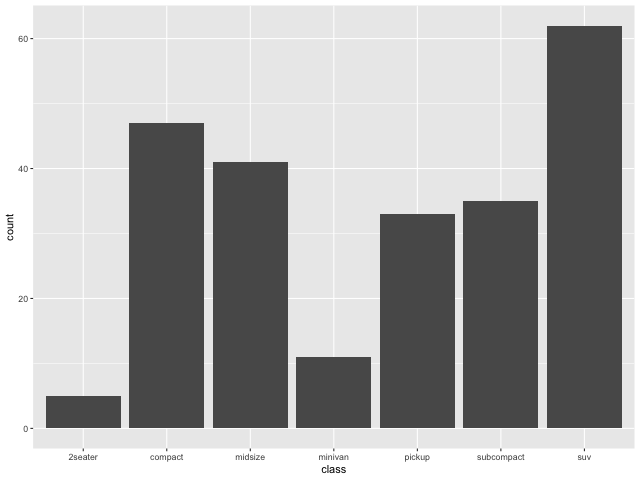
\includegraphics[width=.9\linewidth]{./resources/mpg1.png}
\end{center}
\end{org}

\begin{verbatim}
mpg_summary <- mpg %>%
  group_by(manufacturer) %>%
  summarize(Vehicle_Count=n(), .groups = 'keep') #create summary table
plt <- ggplot(
  mpg_summary,
  aes(x=manufacturer,y=Vehicle_Count)) #import dataset into ggplot2
plt + geom_col()
\end{verbatim}

\begin{org}
\begin{center}
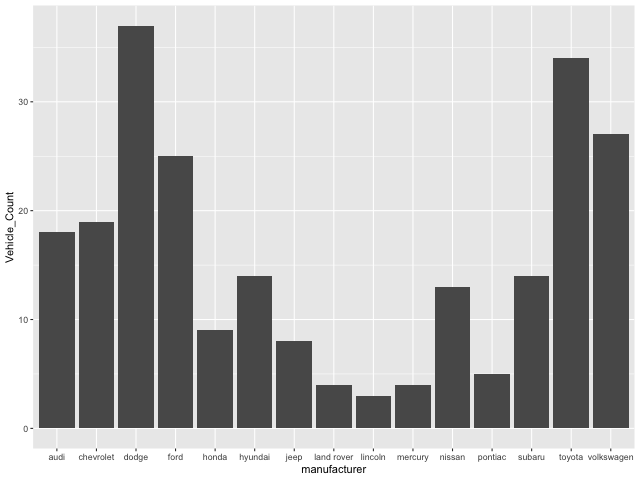
\includegraphics[width=.9\linewidth]{./resources/mpg2.png}
\end{center}
\end{org}

More info at the ggplot2 docs\footnote{\url{https://ggplot2.tidyverse.org/reference/index.html}}.

\subsection{Formatting output}
\label{sec:org8efb858}

Adding labels and themes.

\begin{verbatim}
plt + geom_col() +
  xlab("Manufacturing Company") +
  ylab("Number of Vehicles") +
  theme(axis.text.x=element_text(angle=45, hjust=1))
\end{verbatim}

\begin{org}
\begin{center}
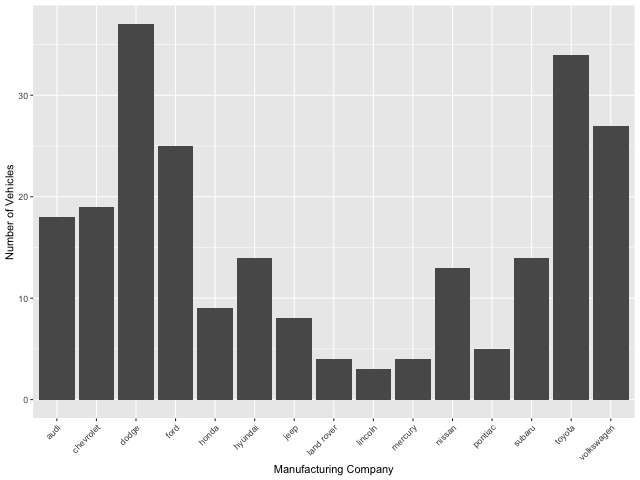
\includegraphics[width=.9\linewidth]{./resources/mpg3.png}
\end{center}
\end{org}

\section{MPG Summary}
\label{sec:org5770c54}

\subsection{Summary Table}
\label{sec:org4abd7cb}

\begin{verbatim}
mpg_summary <-
  subset(mpg, manufacturer=="toyota") %>%
  group_by(cyl) %>%
  summarize(Mean_Hwy=mean(hwy), .groups="keep")
\end{verbatim}

\begin{org}
\begin{center}
\begin{tabular}{rr}
cyl & Mean\textsubscript{Hwy}\\
\hline
4 & 28.2222222222222\\
6 & 22.2307692307692\\
8 & 16.6666666666667\\
\end{tabular}
\end{center}
\end{org}

Import dataset into ggplot and plot the data and adjust the axis.

\begin{verbatim}
plt <- ggplot(mpg_summary, aes(x=cyl, y=Mean_Hwy))
plt + geom_line() +
  scale_x_discrete(limits=c(4, 6, 8)) +
  scale_y_continuous(breaks = c(15:30))
\end{verbatim}

\begin{org}
\begin{center}
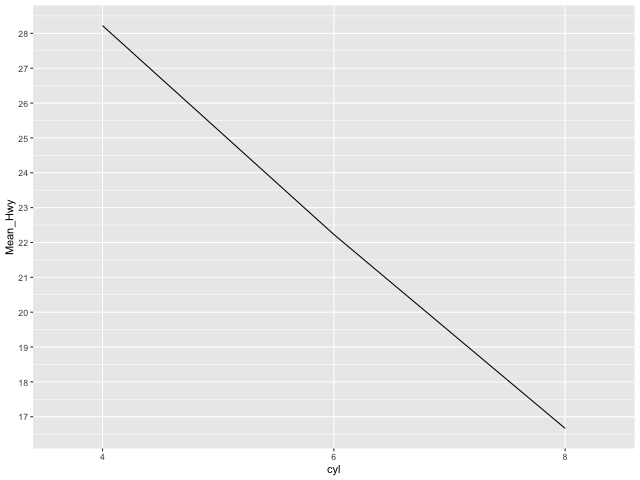
\includegraphics[width=.9\linewidth]{./resources/mpg_summary.png}
\end{center}
\end{org}

\subsection{Mpg dataset}
\label{sec:orgaaad840}

Import into ggplot and plot data with formatting.

\begin{verbatim}
plt <- ggplot(mpg, aes(x=displ, y=cty))
plt + geom_point() +
  xlab("Engine Size (L)") +
  ylab("City Fuel-Efficiency (MPG)")
\end{verbatim}

\begin{org}
\begin{center}
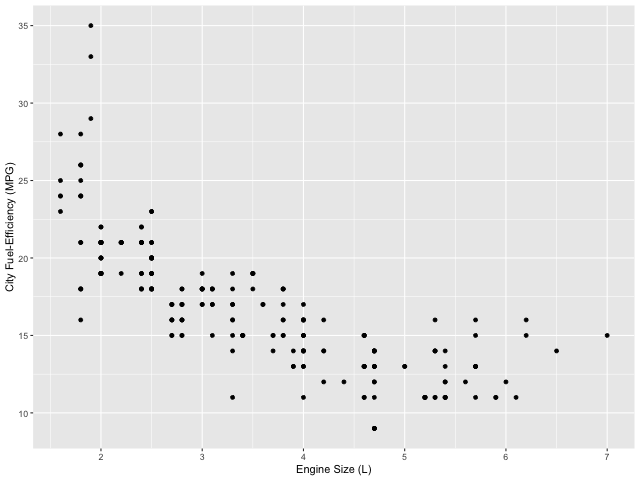
\includegraphics[width=.9\linewidth]{./resources/mpg_dots.png}
\end{center}
\end{org}

Aesthetic changes.

\begin{itemize}
\item alpha changes the transparency of each data point
\item color changes the color of each data point
\item shape changes the shape of each data point
\item size changes the size of each data point
\end{itemize}

\begin{verbatim}
plt <- ggplot(mpg, aes(x=displ, y=cty, color=class))
plt + geom_point() +
  labs(
    x="Engine Size(L)",
    y="City Fuel-Efficiency (MPG)",
    color="Vehicle Class"
)
\end{verbatim}

\begin{org}
\begin{center}
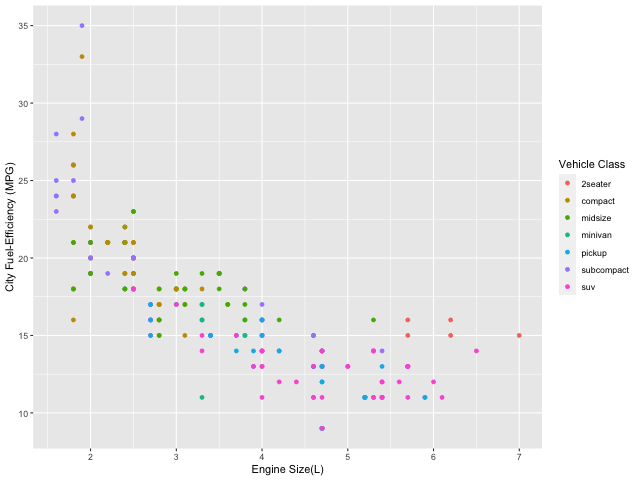
\includegraphics[width=.9\linewidth]{./resources/mpg_dots2.png}
\end{center}
\end{org}

Different shapes.\footnote{\url{https://ggplot2.tidyverse.org/reference/geom\_point.html\#aesthetics}}

\begin{verbatim}
plt <- ggplot(
  mpg,
  aes(x=displ, y=cty, color=class, shape=drv, size=cty)
)
plt + geom_point() +
  labs(
    x="Engine Size (L)",
    y="City Fuel-Efficiency (MPG)",
    color="Vehicle Class",
    shape="Type of Drive"
)
\end{verbatim}

\begin{org}
\begin{center}
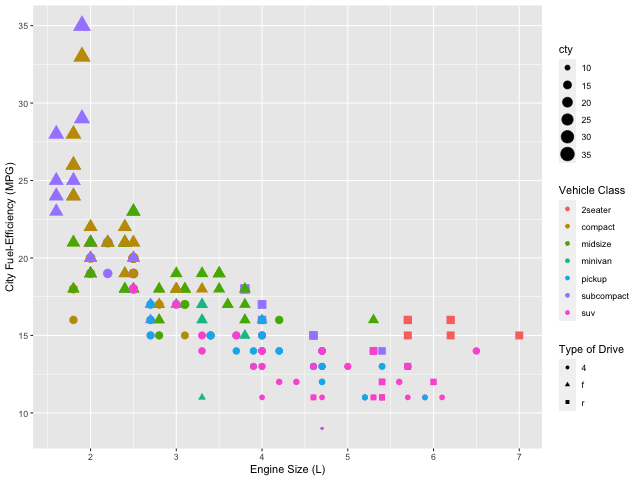
\includegraphics[width=.9\linewidth]{./resources/mpg_dots3.png}
\end{center}
\end{org}

Although there is no technical limit to the number of variables we can add to a ggplot figure, there are diminishing returns. A good rule of thumb is to limit the number of variables displayed in a single figure to a maximum of 3 or 4.

\section{Boxplot}
\label{sec:org05e5add}

Unlike the previous ggplot objects, geom\textsubscript{boxplot}()expects a numeric vector assigned to the y-value\footnote{\url{https://ggplot2.tidyverse.org/reference/geom\_boxplot.html\#aesthetics}}.

\begin{verbatim}
plt <- ggplot(mpg, aes(y=hwy))
plt + geom_boxplot()
\end{verbatim}

\begin{org}
\begin{center}
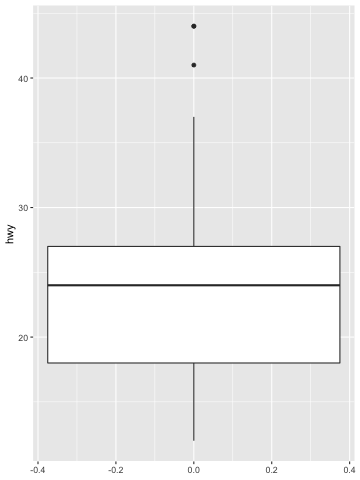
\includegraphics[width=.9\linewidth]{./resources/mpg_box1.png}
\end{center}
\end{org}

Creating multiple boxes.

\begin{verbatim}
plt <- ggplot(mpg, aes(x=manufacturer, y=hwy))
plt +
  geom_boxplot() +
  theme(axis.text.x=element_text(angle=45, hjust=1))
\end{verbatim}

\begin{org}
\begin{center}
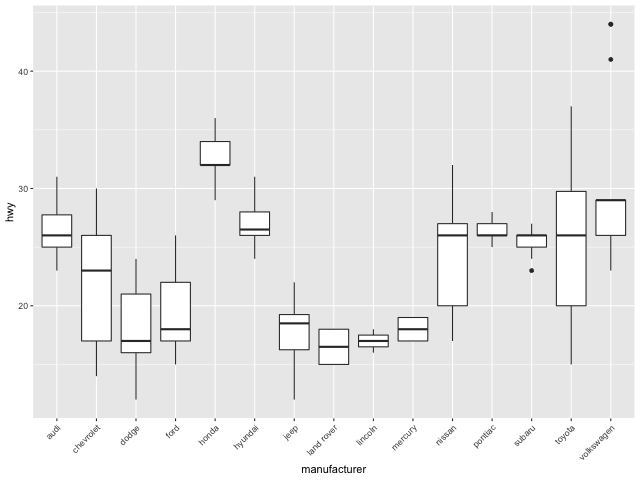
\includegraphics[width=.9\linewidth]{./resources/mpg_box2.png}
\end{center}
\end{org}

\section{Heatmaps}
\label{sec:org74e59e4}

Heatmap plots help visualize the relationship between one continuous numerical variable and two other variables (categorical or numerical).

\subsection{Class and Year Summary}
\label{sec:org7a11ba3}

\begin{verbatim}
mpg_summary <- mpg %>%
  group_by(class, year) %>%
  summarize(Mean_Hwy=mean(hwy), .groups='keep')
\end{verbatim}

\begin{org}
\begin{center}
\begin{tabular}{lrr}
class & year & Mean\textsubscript{Hwy}\\
\hline
2seater & 1999 & 24.5\\
2seater & 2008 & 25\\
compact & 1999 & 27.92\\
compact & 2008 & 28.7272727272727\\
midsize & 1999 & 26.5\\
midsize & 2008 & 28.047619047619\\
minivan & 1999 & 22.5\\
minivan & 2008 & 22.2\\
pickup & 1999 & 16.8125\\
pickup & 2008 & 16.9411764705882\\
subcompact & 1999 & 29\\
subcompact & 2008 & 27.125\\
suv & 1999 & 17.551724137931\\
suv & 2008 & 18.6363636363636\\
\end{tabular}
\end{center}
\end{org}

Plotting heatmap.

\begin{verbatim}
plt <- ggplot(
  mpg_summary,
  aes(x=class, y=factor(year), fill=Mean_Hwy))
plt + geom_tile() +
  labs(
    x="Vehicle Class",
    y="Vehicle Year",
    fill="Mean Highway (MPG)")
\end{verbatim}

\begin{org}
\begin{center}
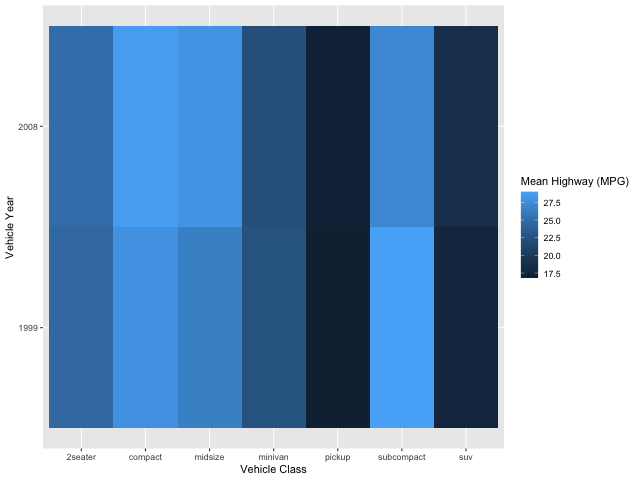
\includegraphics[width=.9\linewidth]{./resources/mpg_heatmap1.png}
\end{center}
\end{org}

\subsection{Model and Year Summary}
\label{sec:org6b768b5}

\begin{verbatim}
mpg_summary <- mpg %>%
  group_by(model, year) %>%
  summarize(Mean_Hwy=mean(hwy), .groups='keep')
mpg_summary %>% head
\end{verbatim}

\begin{org}
\begin{center}
\begin{tabular}{lrr}
model & year & Mean\textsubscript{Hwy}\\
\hline
4runner 4wd & 1999 & 19\\
4runner 4wd & 2008 & 18.5\\
a4 & 1999 & 27.5\\
a4 & 2008 & 29.3333333333333\\
a4 quattro & 1999 & 25.25\\
a4 quattro & 2008 & 26.25\\
\end{tabular}
\end{center}
\end{org}

Adding labels to heatmap.

\begin{verbatim}
plt <- ggplot(
  mpg_summary,
  aes(
    x=model,
    y=factor(year),
    fill=Mean_Hwy)
)
plt + geom_tile() +
  labs(
    x="Model",
    y="Vehicle Year",
    fill="Mean Highway(MPG)"
) +
  theme(
    axis.text.x = element_text(
      angle=90,
      hjust=1,
      vjust=0.5
    )
)
\end{verbatim}

\begin{org}
\begin{center}
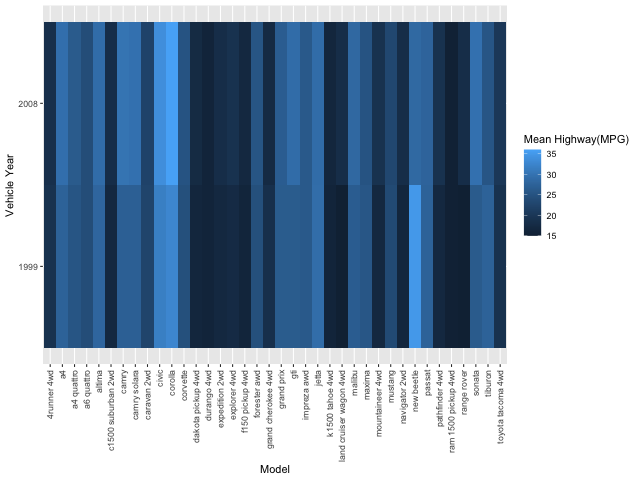
\includegraphics[width=.9\linewidth]{./resources/mpg_heatmap2.png}
\end{center}
\end{org}

We can always refer to the ggplot cheatsheet\footnote{\url{https://github.com/rstudio/cheatsheets/blob/main/data-visualization.pdf}}.

\section{Layered Plots}
\label{sec:org78f78d9}

There are two types of plot layers:

\begin{enumerate}
\item Layering additional plots that use the same variables and input data as the original plot
\item Layering of additional plots that use different but complementary data to the original plot
\end{enumerate}

\begin{verbatim}
plt <- ggplot(mpg, aes(x=manufacturer,y=hwy))
\end{verbatim}

\begin{org}
\begin{center}
\begin{tabular}{}
\hline
\end{tabular}
\end{center}
\end{org}

\begin{verbatim}
plt + geom_boxplot() +
  theme(axis.text.x=element_text(angle=45,hjust=1)) +
  geom_point()
\end{verbatim}

\begin{org}
\begin{center}
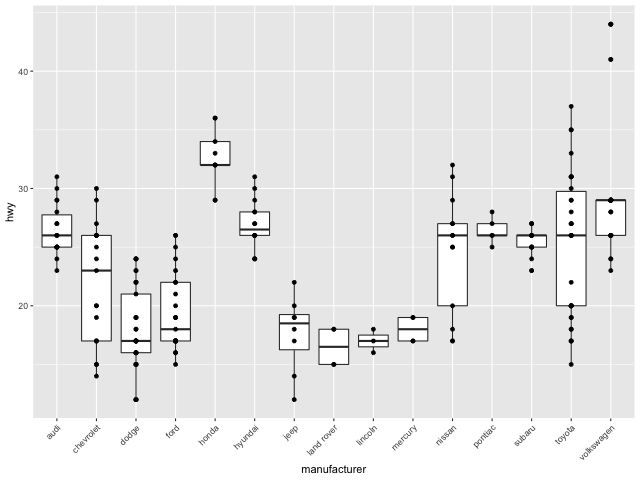
\includegraphics[width=.9\linewidth]{./resources/mpg_layer1.png}
\end{center}
\end{org}

By layering our data points on top of our boxplot, we can see the general distribution of values within each box as well as the number of data points.

\subsection{Summary of Class}
\label{sec:org5cac4ed}

\begin{verbatim}
mpg_summary <- mpg %>%
  group_by(class) %>%
  summarize(Mean_Engine=mean(displ), .groups='keep')
\end{verbatim}

\begin{org}
\begin{center}
\begin{tabular}{lr}
class & Mean\textsubscript{Engine}\\
\hline
2seater & 6.16\\
compact & 2.32553191489362\\
midsize & 2.9219512195122\\
minivan & 3.39090909090909\\
pickup & 4.41818181818182\\
subcompact & 2.66\\
suv & 4.45645161290323\\
\end{tabular}
\end{center}
\end{org}

Plotting scatter plot.

\begin{verbatim}
plt <-
  ggplot(mpg_summary, aes(x=class,y=Mean_Engine))
plt +
  geom_point(size=4) +
  labs(x="Vehicle Class",y="Mean Engine Size")
\end{verbatim}

\begin{org}
\begin{center}
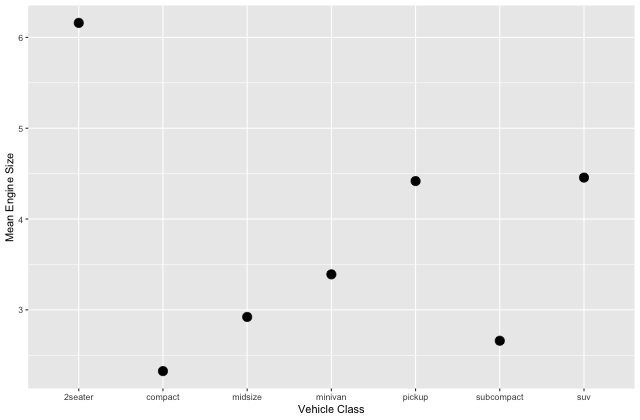
\includegraphics[width=.9\linewidth]{./resources/mpg_layer2.png}
\end{center}
\end{org}

\subsection{Plotting Error Bars}
\label{sec:orgad1a2b4}

Summary of Mean and Standard Deviation of Vehicle Class.

\begin{verbatim}
mpg_summary <-
  mpg %>%
  group_by(class) %>%
  summarize(Mean_Engine=mean(displ), SD_Engine=sd(displ), .groups='keep')
\end{verbatim}

\begin{org}
\begin{center}
\begin{tabular}{lrr}
class & Mean\textsubscript{Engine} & SD\textsubscript{Engine}\\
\hline
2seater & 6.16 & 0.531977443130815\\
compact & 2.32553191489362 & 0.452273524927782\\
midsize & 2.9219512195122 & 0.71850963637308\\
minivan & 3.39090909090909 & 0.452668853478004\\
pickup & 4.41818181818182 & 0.828573527762679\\
subcompact & 2.66 & 1.10245714869372\\
suv & 4.45645161290323 & 1.06580547047714\\
\end{tabular}
\end{center}
\end{org}

Plotting.

\begin{verbatim}
plt <-
  ggplot(mpg_summary, aes(x=class,y=Mean_Engine))
plt +
  geom_point(size=4) +
  labs(x="Vehicle Class", y="Mean Engine Size") +
  geom_errorbar(aes(ymin=Mean_Engine-SD_Engine, ymax=Mean_Engine+SD_Engine))
\end{verbatim}

\begin{org}
\begin{center}
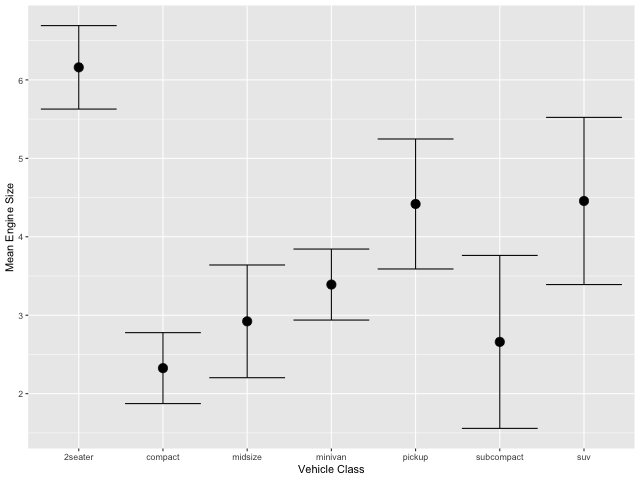
\includegraphics[width=.9\linewidth]{./resources/mpg_layer3.png}
\end{center}
\end{org}

\subsection{Faceting}
\label{sec:orgbc3641c}

Often when our data is in a long format, we want to avoid visualizing all data within a single plot. Rather, we want to plot all our measurements but keep each level (or category) of our grouping variable separate.

Using gather for converting to long format.\footnote{\url{https://tidyr.tidyverse.org/reference/gather.html}}

\begin{verbatim}
mpg_long <-
  mpg %>% gather(key="MPG_Type", value="Rating", c(cty,hwy))
head(mpg_long)
\end{verbatim}

\begin{org}
\begin{center}
\begin{tabular}{llrrrlllllr}
manufacturer & model & displ & year & cyl & trans & drv & fl & class & MPG\textsubscript{Type} & Rating\\
\hline
audi & a4 & 1.8 & 1999 & 4 & auto(l5) & f & p & compact & cty & 18\\
audi & a4 & 1.8 & 1999 & 4 & manual(m5) & f & p & compact & cty & 21\\
audi & a4 & 2 & 2008 & 4 & manual(m6) & f & p & compact & cty & 20\\
audi & a4 & 2 & 2008 & 4 & auto(av) & f & p & compact & cty & 21\\
audi & a4 & 2.8 & 1999 & 6 & auto(l5) & f & p & compact & cty & 16\\
audi & a4 & 2.8 & 1999 & 6 & manual(m5) & f & p & compact & cty & 18\\
\end{tabular}
\end{center}
\end{org}

Plotting many boxplots and coloring by MG type.
\begin{verbatim}
plt <-
  ggplot(mpg_long, aes(x=manufacturer,y=Rating,color=MPG_Type))
plt +
  geom_boxplot() +
  theme(axis.text.x=element_text(angle=45,hjust=1))
\end{verbatim}

\begin{org}
\begin{center}
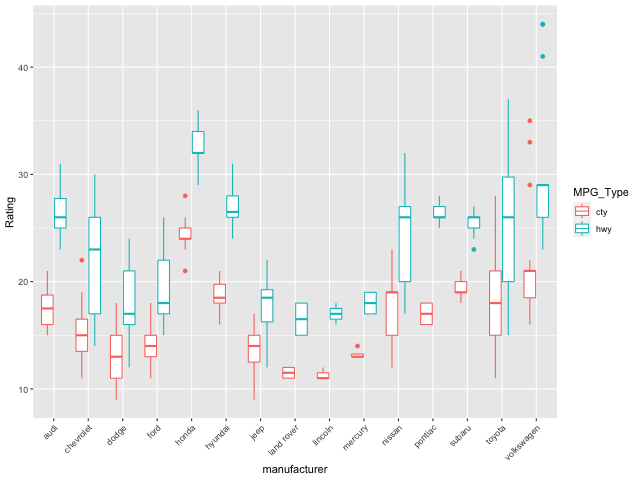
\includegraphics[width=.9\linewidth]{./resources/mpg_faceting.png}
\end{center}
\end{org}

One solution would be to facet the different types of fuel efficiency within the visualization using the facet\textsubscript{wrap}() function\footnote{\url{https://ggplot2-book.org/facet.html}}.

\subsection{Facet Wrap}
\label{sec:org9c517c6}

By faceting our boxplots by fuel-efficiency type, it's easier to make comparisons across manufacturers.

\begin{verbatim}
plt <-
  ggplot(mpg_long,aes(x=manufacturer,y=Rating,color=MPG_Type))
plt +
  geom_boxplot() +
  facet_wrap(vars(MPG_Type)) +
  theme(axis.text.x=element_text(angle=45,hjust=1), legend.position = "none") +
  xlab("Manufacturer")
\end{verbatim}

\begin{org}
\begin{center}
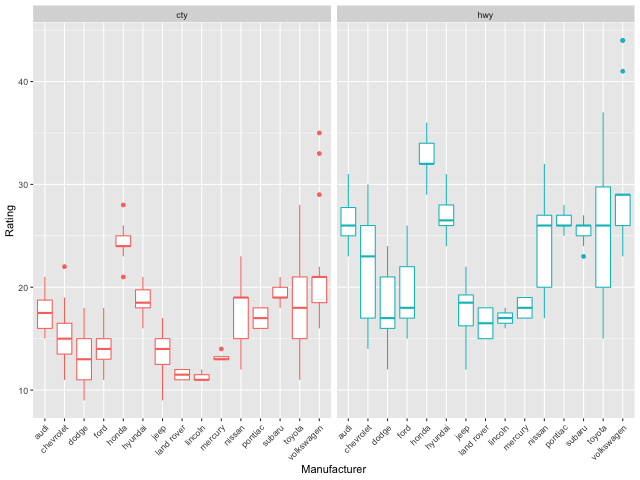
\includegraphics[width=.9\linewidth]{./resources/mpg_facetwrap.png}
\end{center}
\end{org}

Using multiple variables for facet wrap can lead to too many different figures.

\begin{verbatim}
plt <-
  ggplot(mpg_long, aes(x=class, y=Rating, color=class))
plt +
  geom_boxplot() +
  facet_wrap(vars(class)) +
  theme(
    axis.text.x=element_text(angle=45,hjust=1),
    legend.position = "none") +
  xlab("Class")
\end{verbatim}

\begin{org}
\begin{center}
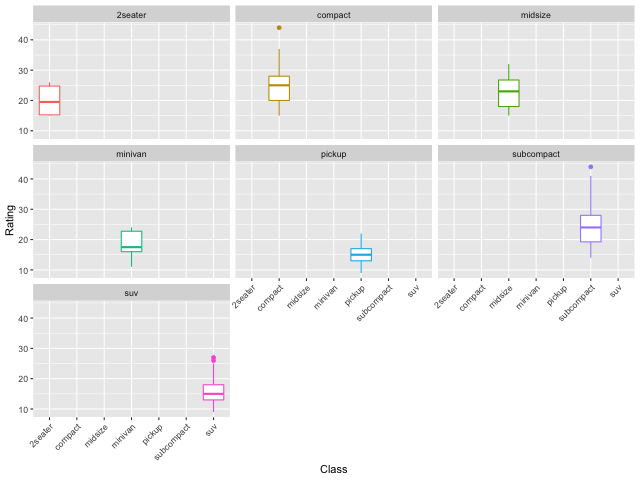
\includegraphics[width=.9\linewidth]{./resources/mpg_facetwrap2.png}
\end{center}
\end{org}
\end{document}
